% Copyright 2006 by Till Tantau
%
% This file may be distributed and/or modified
%
% 1. under the LaTeX Project Public License and/or
% 2. under the GNU Free Documentation License.
%
% See the file doc/generic/pgf/licenses/LICENSE for more details.


\section{Creating Plots}
\label{section-plots}

This section describes the |plot| module.

\begin{pgfmodule}{plot}
    This module provides a set of commands that are intended to make it
    reasonably easy to plot functions using \pgfname. It is loaded
    automatically by |pgf|, but you can load it manually if you have only
    included |pgfcore|.
\end{pgfmodule}


\subsection{Overview}

There are different reasons for using \pgfname\ for creating plots rather than
some more powerful program such as \textsc{gnuplot} or \textsc{mathematica}, as
discussed in Section~\ref{section-why-pgname-for-plots}. So, let us assume that
-- for whatever reason -- you wish to use \pgfname\ for generating a plot.

\pgfname\ (conceptually) uses a two-stage process for generating plots. First,
a \emph{plot stream} must be produced. This stream consists (more or less) of a
large number of coordinates. Second a \emph{plot handler} is applied to the
stream. A plot handler ``does something'' with the stream. The standard handler
will issue line-to operations to the coordinates in the stream. However, a
handler might also try to issue appropriate curve-to operations in order to
smooth the curve. A handler may even do something else entirely, like writing
each coordinate to another stream, thereby duplicating the original stream.

Both for the creation of streams and the handling of streams different sets of
commands exist. The commands for creating streams start with |\pgfplotstream|,
the commands for setting the handler start with |\pgfplothandler|.


\subsection{Generating Plot Streams}

\subsubsection{Basic Building Blocks of Plot Streams}

A \emph{plot stream} is a (long) sequence of the following commands:
%
\begin{enumerate}
    \item |\pgfplotstreamstart|,
    \item |\pgfplotstreampoint|,
    \item |\pgfplotstreampointoutlier|,
    \item |\pgfplotstreampointundefined|,
    \item |\pgfplotstreamnewdataset|,
    \item |\pgfplotstreamspecial|, and
    \item |\pgfplotstreamend|.
\end{enumerate}
%
Between calls of these commands arbitrary other code may be called. Obviously,
the stream should start with the first command and end with the last command.
Here is an example of a plot stream:
%
\begin{codeexample}[code only]
\pgfplotstreamstart
\pgfplotstreampoint{\pgfpoint{1cm}{1cm}}
\newdimen\mydim
\mydim=2cm
\pgfplotstreampoint{\pgfpoint{\mydim}{2cm}}
\advance \mydim by 3cm
\pgfplotstreampoint{\pgfpoint{\mydim}{2cm}}
\pgfplotstreamend
\end{codeexample}

Streams are \emph{global}, meaning that they are not influenced by \TeX\
groups.

\begin{command}{\pgfplotstreamstart}
    This command signals that a plot stream starts. The effect of this command
    is to call the internal command |\pgf@plotstreamstart|, which is set by the
    current plot handler to do whatever needs to be done at the beginning of
    the plot. It will also reset the meaning of the internal commands like
    |\pgf@plotstreampoint| to the initial setting for the plot handler (what
    this means will be explained in a moment).
\end{command}

\begin{command}{\pgfplotstreampoint\marg{point}}
    This command adds a \meta{point} to the current plot stream. The effect of
    this command is to call the internal command |\pgf@plotstreampoint|, which
    is also set by the current plot handler. This command should now ``handle''
    the point in some sensible way. For example, a line-to command might be
    issued for the point.

    When a plot handler is installed, it will setup the internal command
    |\pgf@plotstreampoint| in some way. It is permissible to change the meaning
    of this internal command during a stream. For instance, a handler might
    setup |\pgf@plotstreampoint| in some sensible way for the first point and
    then redefine it so that subsequent points are handled in some other way.

    As mentioned earlier, the |\pgfplotstreamstart| will always reset the
    definition of the internal command to the initial meaning it had when the
    handler was installed. This is true for the other commands mentioned in the
    following.
\end{command}

\begin{command}{\pgfplotstreampointoutlier\marg{point}}
    An \emph{outlier} is a point that is ``out of bounds'' in some way. For
    instance, it might have very large coordinates or the coordinates might
    just be outside some specified range. Nevertheless, an outlier is still a
    well-defined point. This command is issued, for instance, by
    \textsc{gnuplot} when a value is outside the specified range.

    You can configure how outliers are treated using the following key:
    %
    \begin{key}{/pgf/handle outlier points in plots=\meta{how} (initially jump)}
    \keyalias{tikz}
        You can set \meta{how} to one of the following values:
        %
        \begin{itemize}
            \item |plot| This will cause the outlier to be drawn normally, just
                as if |\pgfplotstreampoint| had been used rather than this
                command.
            \item |ignore| The outlier will be completely ignored, just as if
                the command had not been used at all.
            \item |jump| This causes the internal macro |\pgf@plotstreamjump|
                to be called. A ``jump'' in a stream is a position where a
                ``gap'' is introduced. For instance, a simple line-to plot
                handler will stop the current subpath at a jump position and
                begin with a move-to operation at the next normal point of the
                stream.

                The net effect of this setting is that at outlier points plots
                get interrupted and ``restarted'' when the points are no longer
                outliers. This is usually the behaviour you will be looking
                for.
        \end{itemize}
    \end{key}
\end{command}

\begin{command}{\pgfplotstreampointundefined}
    This command indicated that the stream contains an ``undefined'' point like
    a point where some coordinate results for a division by zero. Such a point
    cannot be plotted, which is why it is not given as a parameter. However,
    such a point \emph{can} result in a jump in the plot, depending on the
    setting of the following key:
    %
    \begin{key}{/pgf/handle undefined points in plots=\meta{how} (initially jump)}
    \keyalias{tikz}
        You can set \meta{how} to one of the following values:
        %
        \begin{itemize}
            \item |ignore| The undefined point will be completely ignored, just
                as if the command had not been used at all.
            \item |jump| This causes the internal macro |\pgf@plotstreamjump|
                to be called.
        \end{itemize}
    \end{key}
\end{command}

\begin{command}{\pgfplotstreamnewdataset}
    This command indicated that in the stream a ``new data set'' starts. So,
    the stream does not end, but there is a logical break in the data. For
    example, when a table is read from a file, empty lines are interpreted as
    indicating new data sets. What happens when a new data set is encountered
    is governed by the following key:
    %
    \begin{key}{/pgf/handle new data sets in plots=\meta{how} (initially jump)}
    \keyalias{tikz}
        You can set \meta{how} to one of the following values:
        %
        \begin{itemize}
            \item |ignore| The command will be completely ignored, just as if
                the command had not been used at all.
            \item |jump| This causes the internal macro |\pgf@plotstreamjump|
                to be called.
        \end{itemize}
    \end{key}
\end{command}

\begin{command}{\pgfplotstreamspecial\marg{text}}
    This command causes |\pgf@plotstreamspecial| to be called with \meta{text}
    as its parameter. This allows handler-specific information to be passed to
    the handler. All normal handlers ignore this command.
\end{command}

\begin{command}{\pgfplotstreamend}
    This command signals that a plot stream ends. It calls
    |\pgf@plotstreamend|, which should now do any necessary ``cleanup''.
\end{command}

Note that plot streams are not buffered, that is, the different points are
handled immediately. However, using the recording handler, it is possible to
record a stream.


\subsubsection{Commands That Generate Plot Streams}
\label{section-plot-jumps}

Plot streams can be created ``by hand'' as in the earlier example. However,
most of the time the coordinates will be produced internally by some command.
For example, the |\pgfplotxyfile| reads a file and converts it into a plot
stream.

\begin{command}{\pgfplotxyfile\marg{filename}}
    This command will try to open the file \meta{filename}. If this succeeds,
    it will convert the file contents into a plot stream as follows: A
    |\pgfplotstreamstart| is issued. Then, for each empty line a
    |\pgfplotstreamnewdataset| is produced. Other lines in the file should
    start with two numbers separated by a space, such as |0.1 1| or |100 -.3|.
    The numbers may be followed by some text, which will be ignore
    \emph{except} if it is exactly ``|u|'' or ``|o|''. For ``|u|'' the point
    is considered to be undefined and |\pgfplotstreampointundefined| is called.
    For ``|o|'' the point is considered to be an outlier and
    |\pgfplotstreampointoutlier| is called. Otherwise, each pair \meta{x} and
    \meta{y} of numbers is converted into one plot stream point in the
    $xy$-coordinate system. Thus, a line like
    %
\begin{codeexample}[code only, tikz syntax=false]
0 Nan u
1 1 some text
2 4
3 9

4 16 o
5 25 oo
\end{codeexample}
    %
    is turned into
    %
\begin{codeexample}[code only]
\pgfplotstreamstart
\pgfplotstreampointundefined
\pgfplotstreampoint{\pgfpointxy{1}{1}}
\pgfplotstreampoint{\pgfpointxy{2}{4}}
\pgfplotstreampoint{\pgfpointxy{3}{9}}
\pgfplotstreamnewdataset
\pgfplotstreampointoutlier{\pgfpointxy{4}{16}}
\pgfplotstreampoint{\pgfpointxy{5}{25}}
\pgfplotstreamend
\end{codeexample}
    %
    (Note that the last line is not an outlier because |oo| is not the same as
    |o|).

    The two characters |%| and |#| are also allowed in a file and they are both
    treated as comment characters. Thus, a line starting with either of them is
    treated as empty.

    When the file has been read completely, |\pgfplotstreamend| is called.
\end{command}

\begin{command}{\pgfplotxyzfile\marg{filename}}
    This command works like |\pgfplotxyfile|, only \emph{three} numbers are
    expected on each non-empty line. They are converted into points in the
    $xyz$-coordinate system. Consider, the following file:
    %
\begin{codeexample}[code only, tikz syntax=false]
% Some comments
# more comments
2 -5  1 first entry
2 -.2 2 o
2 -5  2 third entry
\end{codeexample}
    %
    It is turned into the following stream:
    %
\begin{codeexample}[code only]
\pgfplotstreamstart
\pgfplotstreamnewdataset
\pgfplotstreamnewdataset
\pgfplotstreampoint{\pgfpointxyz{2}{-5}{1}}
\pgfplotstreampointoutlier{\pgfpointxyz{2}{-.2}{2}}
\pgfplotstreampoint{\pgfpointxyz{2}{-5}{2}}
\pgfplotstreamend
\end{codeexample}
    %
\end{command}

Currently, there is no command that can decide automatically whether the
$xy$-coordinate system should be used or whether the $xyz$-system should be
used. However, it would not be terribly difficult to write a ``smart file
reader'' that parses coordinate files a bit more intelligently.

\begin{command}{\pgfplotfunction\marg{variable}\marg{sample list}\marg{point}}
    This command will produce coordinates by iterating the \meta{variable} over
    all values in \meta{sample list}, which should be a list in the |\foreach|
    syntax. For each value of \meta{variable}, the \meta{point} is evaluated
    and the resulting coordinate is inserted into the plot stream.
    %
\begin{codeexample}[]
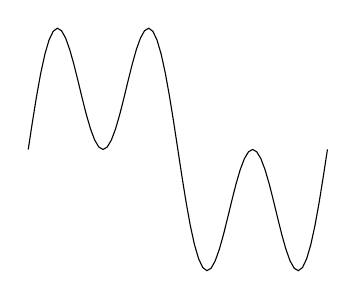
\begin{tikzpicture}[x=3.8cm/360]
  \pgfplothandlerlineto
  \pgfplotfunction{\x}{0,5,...,360}{\pgfpointxy{\x}{sin(\x)+sin(3*\x)}}
  \pgfusepath{stroke}
\end{tikzpicture}
\end{codeexample}

\begin{codeexample}[]
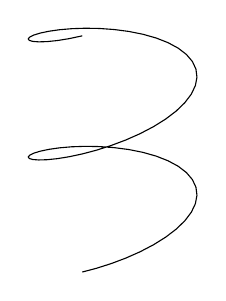
\begin{tikzpicture}[y=3cm/360]
  \pgfplothandlerlineto
  \pgfplotfunction{\y}{0,5,...,360}{\pgfpointxyz{sin(2*\y)}{\y}{cos(2*\y)}}
  \pgfusepath{stroke}
\end{tikzpicture}
\end{codeexample}

    Be warned that if the expressions that need to evaluated for each point are
    complex, then this command can be very slow.
\end{command}

\begin{command}{\pgfplotgnuplot\oarg{prefix}\marg{function}}
    This command will ``try'' to call the \textsc{gnuplot} program to generate
    the coordinates of the \meta{function}. In detail, the following happens:

    This command works with two files: \meta{prefix}|.gnuplot| and
    \meta{prefix}|.table|.  If the optional argument \meta{prefix} is not
    given, it is set to |\jobname|.

    Let us start with the situation where none of these files exists. Then
    \pgfname\ will first generate the file \meta{prefix}|.gnuplot|. In this
    file it writes
    %
\begin{codeexample}[code only, tikz syntax=false]
set terminal table; set output "#1.table"; set format "%.5f"
\end{codeexample}
    %
    where |#1| is replaced by \meta{prefix}. Then, in a second line, it writes
    the text \meta{function}.

    Next, \pgfname\ will try to invoke the program |gnuplot| with the argument
    \meta{prefix}|.gnuplot|. This call may or may not succeed, depending on
    whether the |\write18| mechanism (also known as shell escape) is switched
    on and whether the |gnuplot| program is available.

    Assuming that the call succeeded, the next step is to invoke
    |\pgfplotxyfile| on the file \meta{prefix}|.table|; which is exactly the
    file that has just been created by |gnuplot|.
    %
\begin{codeexample}[]
\begin{tikzpicture}
  \draw[help lines] (0,-1) grid (4,1);
  \pgfplothandlerlineto
  \pgfplotgnuplot[plots/pgfplotgnuplot-example]{plot [x=0:3.5] x*sin(x)}
  \pgfusepath{stroke}
\end{tikzpicture}
\end{codeexample}

    The more difficult situation arises when the |.gnuplot| file exists, which
    will be the case on the second run of \TeX\ on the \TeX\ file. In this case
    \pgfname\ will read this file and check whether it contains exactly what
    \pgfname\ ``would have written'' into this file. If this is not the case,
    the file contents is overwritten with what ``should be there'' and, as
    above, |gnuplot| is invoked to generate a new |.table| file. However, if
    the file contents is ``as expected'', the external |gnuplot| program is
    \emph{not} called. Instead, the \meta{prefix}|.table| file is immediately
    read.

    As explained in Section~\ref{section-tikz-gnuplot}, the net effect of the
    above mechanism is that |gnuplot| is called as seldom as possible and that
    when you pass along the |.gnuplot| and |.table| files with your |.tex| file
    to someone else, that person can \TeX\ the |.tex| file without having
    |gnuplot| installed and without having the |\write18| mechanism switched
    on.

    \begin{key}{/pgf/plot/gnuplot call=\meta{gnuplot invocation} (initially gnuplot)}
        This key can be used to change the way gnuplot is called.

        Some portable MiK\TeX{} distribution needs something like the
        following.
        %
\begin{codeexample}[code only]
  \pgfkeys{/pgf/plot/gnuplot call="/Programs/gnuplot/binary/gnuplot"}
\end{codeexample}
    \end{key}
\end{command}


\subsection{Plot Handlers}
\label{section-plot-handlers}

A \emph{plot handler}  determines what ``should be done'' with a plot stream.
You must set the plot handler before the stream starts. The following commands
install the most basic plot handlers; more plot handlers are defined in the
file |pgflibraryplothandlers|, which is documented in
Section~\ref{section-library-plothandlers}.

All plot handlers work by setting or redefining the following three macros:
|\pgf@plotstreamstart|, |\pgf@plotstreampoint|, and |\pgf@plotstreamend|.

\begin{command}{\pgfplothandlerlineto}
    This handler will issue a |\pgfpathlineto| command for each point of the
    plot, \emph{except} possibly for the first. What happens with the first
    point can be specified using the two commands described below.
    %
\begin{codeexample}[]
\begin{pgfpicture}
  \pgfpathmoveto{\pgfpointorigin}
  \pgfplothandlerlineto
  \pgfplotstreamstart
  \pgfplotstreampoint{\pgfpoint{1cm}{0cm}}
  \pgfplotstreampoint{\pgfpoint{2cm}{1cm}}
  \pgfplotstreampoint{\pgfpoint{3cm}{2cm}}
  \pgfplotstreampoint{\pgfpoint{1cm}{2cm}}
  \pgfplotstreamend
  \pgfusepath{stroke}
\end{pgfpicture}
\end{codeexample}
    %
\end{command}

\begin{command}{\pgfsetmovetofirstplotpoint}
    Specifies that the line-to plot handler (and also some other plot handlers)
    should issue a move-to command for the first point of the plot instead of a
    line-to. This will start a new part of the current path, which is not
    always, but often, desirable. This is the default.
\end{command}

\begin{command}{\pgfsetlinetofirstplotpoint}
    Specifies that  plot handlers should issue a line-to command for the first
    point of the plot.
    %
\begin{codeexample}[]
\begin{pgfpicture}
  \pgfpathmoveto{\pgfpointorigin}
  \pgfsetlinetofirstplotpoint
  \pgfplothandlerlineto
  \pgfplotstreamstart
  \pgfplotstreampoint{\pgfpoint{1cm}{0cm}}
  \pgfplotstreampoint{\pgfpoint{2cm}{1cm}}
  \pgfplotstreampoint{\pgfpoint{3cm}{2cm}}
  \pgfplotstreampoint{\pgfpoint{1cm}{2cm}}
  \pgfplotstreamend
  \pgfusepath{stroke}
\end{pgfpicture}
\end{codeexample}
    %
\end{command}

\begin{command}{\pgfplothandlerpolygon}
    This handler works like the line-to plot handler, only the line is closed
    at the end using |\pgfpathclose|, resulting in a polygon.
\end{command}

\begin{command}{\pgfplothandlerdiscard}
    This handler will simply throw away the stream.
\end{command}

\begin{command}{\pgfplothandlerrecord\marg{macro}}
    When this handler is installed, each time a plot stream command is called,
    this command will be appended to \meta{macro}. Thus, at the end of the
    stream, \meta{macro} will contain all the commands that were issued on the
    stream. You can then install another handler and invoke \meta{macro} to
    ``replay'' the stream (possibly many times).
    %
\begin{codeexample}[]
\begin{pgfpicture}
  \pgfplothandlerrecord{\mystream}
  \pgfplotstreamstart
  \pgfplotstreampoint{\pgfpoint{1cm}{0cm}}
  \pgfplotstreampoint{\pgfpoint{2cm}{1cm}}
  \pgfplotstreampoint{\pgfpoint{3cm}{1cm}}
  \pgfplotstreampoint{\pgfpoint{1cm}{2cm}}
  \pgfplotstreamend
  \pgfplothandlerlineto
  \mystream
  \pgfplothandlerclosedcurve
  \mystream
  \pgfusepath{stroke}
\end{pgfpicture}
\end{codeexample}
    %
\end{command}


\subsection{Defining New Plot Handlers}

You can define new plot handlers using the following command:

\begin{command}{\pgfdeclareplothandler\marg{macro}\marg{arguments}\marg{configuration}}
    This command creates a new plot handler that can subsequently be called
    using the macro \meta{macro}. This macro take the arguments given in
    \meta{arguments}, which can be a list like |#1#2| if \meta{macro} should be
    invoked with two arguments. Here is a typical example:
    %
\begin{codeexample}[code only]
\pgfdeclareplothandler{\myhandler}{#1}{...}
...
\myhandler{foo}
\pgfplotstreamstart
...
\pgfplotstreamend
\end{codeexample}

    The \meta{configuration} is used to define the behaviour of the handler. It
    is a list of key--value pairs, where the following keys are allowed:
    %
    \begin{itemize}
        \item |start=|\meta{code}. The \meta{code} will be executed whenever
            |\pgfplotstreamstart| is used while the handler \meta{macro} is
            selected. Inside the \meta{code}, you can use |#1|, |#2|, and so on
            to refer to the parameters that were given to \meta{macro}:
            %
\begin{codeexample}[width=6cm]
\pgfdeclareplothandler{\myhandler}{#1}{
  start = Hi #1.,
  end   = Bye #1.,
}
\myhandler{foo}
\pgfplotstreamstart
\pgfplotstreamend
\myhandler{bar}
\pgfplotstreamstart
\pgfplotstreamend
\end{codeexample}
            %
        \item |end=|\meta{code} Works just like |start|.
        \item |point=|\meta{code}. The \meta{code} will be executed whenever
            |\pgfplotstreampoint| is used while the handler \meta{macro} is in
            force. Inside the \meta{code}, you can use |#1|, |#2|, and so on to
            refer to the arguments give to \meta{macro}, while you can use
            |##1| to refer to the argument given to |\pgfplotstreampoint|
            itself (this will be the coordinate).
            %
\begin{codeexample}[]
\pgfdeclareplothandler{\myhandler}{#1}{
  point=\pgfpathcircle{##1}{#1} % ##1 is the coordinate,
                                % #1 the parameter for \myhandler
}
\begin{pgfpicture}
  \myhandler{1pt}
  \pgfplotstreamstart
  \pgfplotstreampoint{\pgfpoint{0pt}{0pt}}
  \pgfplotstreampoint{\pgfpoint{3pt}{3pt}}
  \pgfplotstreampoint{\pgfpoint{6pt}{3pt}}
  \pgfplotstreampoint{\pgfpoint{9pt}{0pt}}
  \pgfplotstreamend
  \pgfusepath{stroke}
  \myhandler{3pt}
  \pgfplotstreamstart
  \pgfplotstreampoint{\pgfpoint{0pt}{0pt}}
  \pgfplotstreampoint{\pgfpoint{9pt}{0pt}}
  \pgfplotstreamend
  \pgfusepath{stroke}
\end{pgfpicture}
\end{codeexample}
            %
            The \meta{code} will also be called for
            |\pgfplotstreampointoutlier| when this command has been configured
            to |plot| the outliers.
        \item |jump=|\meta{code} The \meta{code} will be called whenever a jump
            has been requested indirectly via an outlier point, and undefined
            point, or a new data set (for each of which the command needs to be
            configured to |jump|). As always, inside the \meta{code} you can
            access |#1| and so on.
        \item |special=|\meta{code} Causes \meta{code} to be executed whenever
            |\pgfplotstreamspecial|\marg{something} is used. Inside the
            \meta{code}, you can access \meta{something} via |##1| and the
            parameters of \meta{macro} as |#1|, |#2|, and so on.
    \end{itemize}

    In addition to the above keys, there exist also ``code macro versions'' of
    them:
    %
    \begin{itemize}
        \item |point macro=|\meta{some macro}. Causes |\pgfplotstreampoint| to
            call \meta{some macro} directly (actually, |\pgf@plotstreampoint|
            is set to be equal to \meta{some macro}). Inside the \meta{some
            macro} you can use |#1| to access the coordinate passed to
            |\pgfplotstreampoint| and you can no longer access the parameters
            passed to the original call to \meta{macro} that installed the
            handler. So, \meta{some macro} must take exactly one argument,
            namely |#1|.
        \item |special macro=|\meta{some macro}. As |point macro|, only for
            specials.
        \item |start macro=|\meta{some macro}. Causes \meta{some macro} to be
            executed at the start. This macro, like the below ones, may not
            take any parameters and will not have access to the parameters
            passed to the original \meta{macro}.
        \item |end macro=|\meta{some macro}. As above.
        \item |jump macro=|\meta{some macro}. As above.
    \end{itemize}
\end{command}


%%% Local Variables:
%%% mode: latex
%%% TeX-master: "pgfmanual"
%%% End:
